\section{Problem Definition}

Event Stream Processing (or shorter \textit{Stream Processing} has become one of the most common computing tasks enterprise systems face today. As defined by the Gartner Research Institute,
\blockquote{An event stream is a sequence of event objects arranged in some order, typically by time. \acf{ESP} is any kind of computing performed on event streams.}\footcite{Schulte2017TechnologyProcessing}\\
In other words, \acf{ESP} processes data \textit{directly} as it is produced by nodes (i.e. applications, sensors, ...). "Event" is often just defined as a "notable thing that happens".\footcite{Michelson2011ElementalOverview} This is a very broad definition that has to be revised and adapted based on the use-case at hand but a shared characteristic is that all events contain information, are generated as a byproduct of the occurrence of something and can be associated with a specific point in time. 
Since many real world scenarios such as sensor measurements, financial trades, and so forth regularly result in a continuous stream of events, \acf{ESP} is often a viable architectural approach.\\
The traditional solution to this challenge is to store the data in a database and let applications query the data as needed or as scheduled. As depicted in \ref{fig:dataRest}, the occurring events are sent from an application or sensor to an endpoint where they are stored at rest and the computation of said events has to be scheduled and managed. It is important to note that the information flow in this model centers around the data storage. First the information flow from the source to it and after that the computation applications have to make some kind of request to it to get access to the information.

\begin{figure}[ht]
    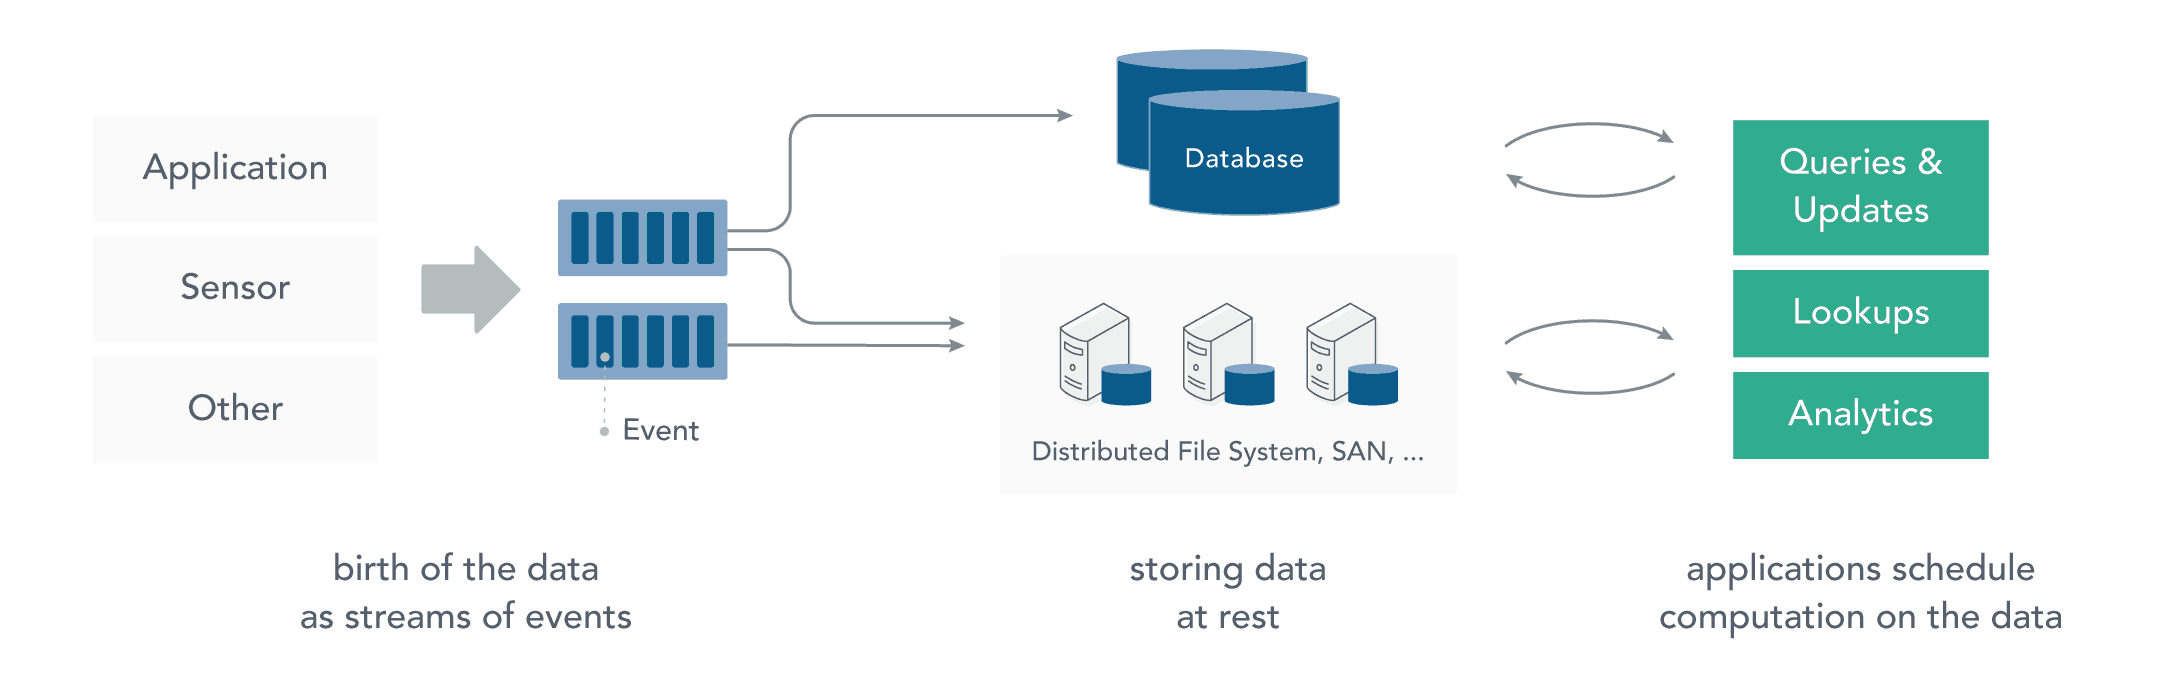
\includegraphics[width=\linewidth]{images/streaming/data_at_rest.png}\centering
    \caption
    [Data-at-Rest Architecture]
    {Data-at-Rest Architecture (\cite{dataArtisansWhatProcessing})}
    \label{fig:dataRest}
\end{figure}

With Stream Processing however, a continuous data flow from left to right is established. Upon receiving an event from the stream, the \acf{ESP} application performs a task based on the event. For instance, this could be a transformation of the events properties in order to match system-wide standards (e.g., unit conversation). 
\ref{fig:dataStream} shows a simplified example of this pattern. Similarly to \ref{fig:dataRest}, applications, sensors or other clients continuously generate events that are sent to an endpoint but instead of storing the data, it is directly processed by the assigned application. As indicated by the two arrows that lead from two streams to one single application, it is likewise possible to process multiple streams jointly and merge information flows. The so-called \textit{stream processors} directly react upon the events as mentioned before. 

\begin{figure}[ht]
    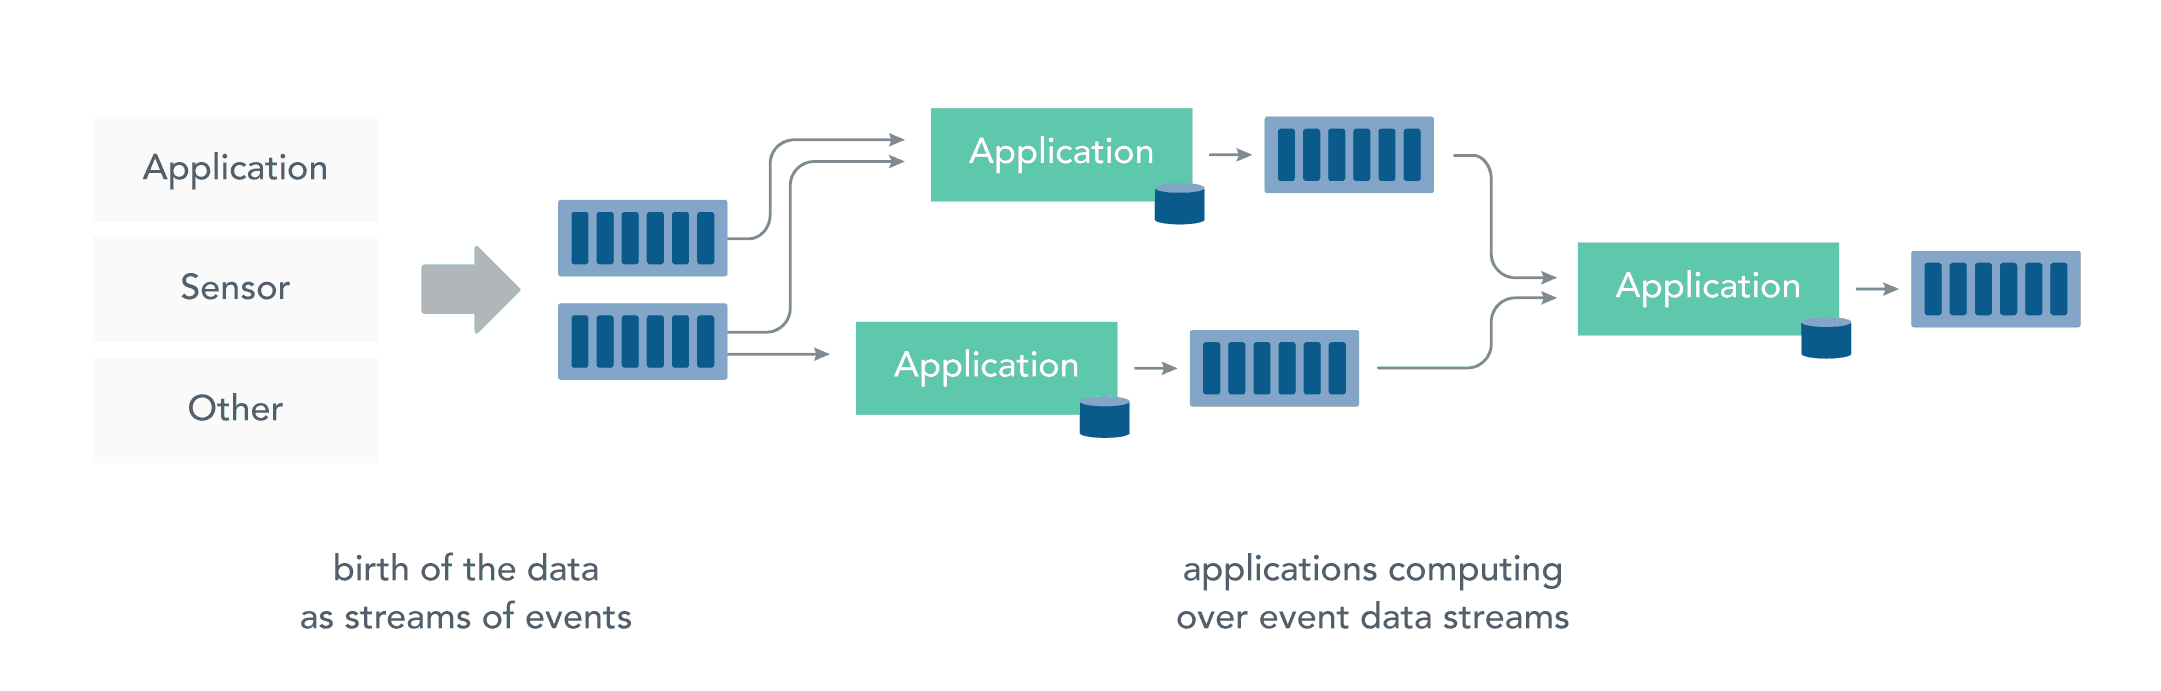
\includegraphics[width=\linewidth]{images/streaming/streming_data.png}\centering
    \caption
    [Stream Processing Architecture]
    {Stream Processing Architecture (\cite{dataArtisansWhatProcessing})}
    \label{fig:dataStream}
\end{figure}

This seemingly small changes to the information flow has some serious implications. To begin with, \acf{ESP} resembles the natural flow of data outside the IT system much closer than scheduled computation and is therefore easier to understand and design. Secondly, since the event is processed immediately upon being received, the application can react instantly and a lag time between the occurrence of the event, the action trigger and the action itself can be avoided which results in a near real-time processing of information. 

This approach allows for a data-driven and computation-driven perspective on complex business problems that aim to provide dynamic insights and need to handle a steady input of information. 
Due to recent trends such as IoT, the amount of data that has to be categorized, analyzed and processed skyrocketed. The data-ingress often consists of semi-structured sets and has to be transformed and handled in near real-time\footcite{Dekate2017PredictsInfrastructure} in order to provide valuable business insights for companies and public sector players alike, suggesting that this approach is not only a temporarily trend but rather a long lasting evolution of the way data-centric enterprise systems are being designed. Moreover, a recent Gartner report predicts that the market for \acf{ESP} solutions will grow by 15\% year over year from 2017 to 2022 (compound annual growth rate).\footcite{Heudecker2017MarketProcessing} 

Traditional approaches such as monolithic on-premise systems and even \acf{PaaS} based solutions or clusters  

"Serverless" computing aims to solve those problems.\footcite{Roberts2016ServerlessArchitectures}

Many companies such as Netflix\footnote{\url{https://aws.amazon.com/solutions/case-studies/netflix-kinesis-streams/}} or Uber\footnote{\url{https://flink.apache.org/poweredby}} adopted stream-processing patterns in combination with serverless computing to take on challenges that demand highly scale able and performant systems. 
This approach is particularly favourable for companies that deliver IoT solutions such as Toyota\footnote{\url{https://aws.amazon.com/solutions/case-studies/toyota-tsusho/}} or Quest\footnote{\url{https://customers.microsoft.com/en-us/story/quest}}.